\section{Modellierung betrieblicher Informationssysteme}

\subsection{Grundlagen der Modellierung}
    \subsubsection*{Definition und Ziele}
        Die Modellierung dient der konsistenten, korrekten und vollständigen Erfassung und Darstellung der Anforderungen an betriebliche Informationssysteme. Ziel ist es, Geschäftsprozesse und unterstützende betriebliche Anwendungen optimal aufeinander abzustimmen.
    \subsubsection*{Charakteristika}
        Ein Modell ist eine vereinfachte und zweckorientierte Abbildung eines realen oder imaginären Sachverhalts.
        \begin{itemize}
            \item Abbildungscharakter: Sicht auf bestimmten Bezugspunkt
            \item Vereinfachung: Modell ist immer „einfacher“ als eigentlicher Sachverhalt
            \item Zweckorientierung: Modell hat immer einen bestimmten Zweck
        \end{itemize}
    \subsubsection*{Prinzipien/Eigenschaften}
        \begin{itemize}
            \item Partitionierung: Zerlegung eines komplexen Sachverhalts in isolierte Teilbereiche
            \item Projektion: Betrachtung eines Sachverhalts aus verschiedenen Perspektiven
            \item Abstraktion: Vernachlässigung unwesentlicher Details zur Fokussierung auf wesentliche Aspekte
        \end{itemize}
    \subsubsection*{Arten von Modellen}
        \begin{itemize}
            \item IST-Modell: Zeigt den aktuellen Zustand (dokumentierend)
            \item SOLL-Modell: Zeigt den geplanten zukünftigen Zustand (entwerfend)
            \item Referenzmodell: Anerkannte Lösungsvorschlag, dient zum Vergleich mit IST und als Vorlage für SOLL
        \end{itemize}

\subsection{Modellierungssprachen}
    \subsubsection*{Definition}
        Modellierungssprachen definieren die Syntax und Semantik für die Erstellung von Modellen.
    \subsubsection*{Beispiele}
        BPMN (Business Process Model and Notation) verwendet spezifische Symbole und Regeln zur Darstellung von Geschäftsprozessen.
    \subsubsection*{Ausdrucksstärke}
        Die Ausdrucksstärke einer Modellierungssprache bestimmt, welche Aspekte eines Sachverhalts dargestellt werden können und wie detailliert diese sind.

\subsection{Grundzüge ordnungsgemäßer Modellierung}
    \subsubsection*{Richtigkeit}
        Modelle müssen den zu modellierender Sachverhalt korrekt abbilden (semantisch und syntaktisch).
    \subsubsection*{Relevanz}
        Modelle sollten alle relevanten Details enthalten und irrelevante Details ausblenden.
    \subsubsection*{Wirtschaftlichkeit}
        Relevante Details sollten nur modelliert werden, wenn deren Erhebung nicht zu aufwendig ist.
    \subsubsection*{Klarheit}
        Modelle müssen verständlich dargestellt werden.
    \subsubsection*{Vergleichbarkeit}
        Vergleichbarkeit: Einheitliche Terminologie und Struktur für Modelle eines Unternehmens.
    \subsubsection*{Systematik}
        Modelle müssen systematisch organisiert sein.

\subsection{Architektur Integrierter Informationssysteme (ARIS)}
    \subsubsection*{Definition}
        ARIS beschreibt die ganzheitliche Struktur eines Unternehmens in Form der verwendeten Prozesse, Organisationsstrukturen, Funktionen, Daten und Kommunikationsbeziehungen.
    \subsubsection*{Ziele}
        Reduktion der Komplexität durch Rahmenwerke wie ARIS, um eine systematische und einheitliche Modellierung zu ermöglichen.
    \begin{figure}[h]
        \centering
        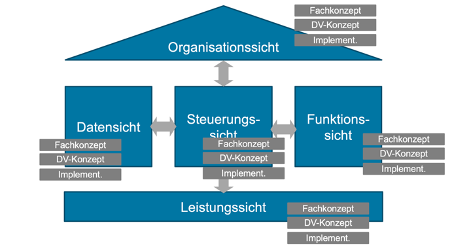
\includegraphics[width=\textwidth]{image/ARIS.png}
        \caption{ARIS}
        \label{fig:ARIS}
    \end{figure}